The objective here is to formalize the notion of \textit{why one grouping of attributes may be better than another ?}. There are 2 levels to measure the goodness of a schema :
\begin{itemize}
    \item The logical (conceptual) level : What is the meaning of the attributes in the relation schema (base + views)
    \item The implementation (physical storage) level : How the tuples are stored and updated (only base)
\end{itemize}

There are 2 methods to deal with normalization :
\begin{itemize}
    \item Bottom-up : Consider the basic relationships and assemble them (not very popular)
    \item Top-down : Start with groupings of attributes, analyzed and decomposed
\end{itemize}
$\Rightarrow$ preserve information + minimum redundancy

\section{Informal Design Guidelines for Relation Schemas}
\subsection{Make sure that the semantics of the attributes is clear in the schema}
Attributes belonging to one relation have a real-world meaning and an interpretation with it.
\begin{center}
Easily explained semantic = better relation database schema
\end{center}

$\Rightarrow$\textbf{Guideline 1 } Design a relation schema so that it is easy to explain its meaning. Do not  combine attributes from various entity types into a single relation.


\subsection{Reduce the redundant information in tuples}
One aim is to minimize the storage used by the base relation. Let's take a look at figure \ref{fig:empdep} which shows two (natural) relations representing the list of employees and the list of departments. If we merge those two relations, we get the relation shown on figure \ref{fig:mixempdep}.\\

\begin{figure}[!h]
    \centering
    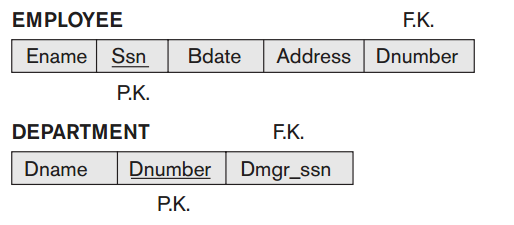
\includegraphics[scale=0.4]{chapter14_emp_dep.png}
    \caption{Employee-department, 2 relations (natural way)}
    \label{fig:empdep}
\end{figure}

\begin{figure}[!h]
    \centering
    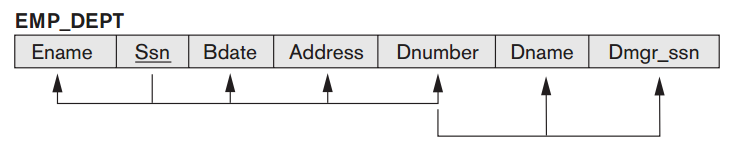
\includegraphics[scale=0.4]{chapter14_mix_emp_dep.png}
    \caption{Employee-department, mixed relations }
    \label{fig:mixempdep}
\end{figure}

In fact, what we will get by using the mixed version, is a severe redundancy of informations. For each employee, the Dname and Dmgr$\_$ssn will be repeated. It means that if 2000 employees are in the same department, the same combination of Dnumber/Dname and Dmgr$\_$ssn will appear 2000 times instead of 1 $\Rightarrow$ Huge redundancy $\Rightarrow$ huge loss of memory + possibility of update anomalies.
\newpage
\subsubsection{Update anomalies}
\begin{itemize}
    \item \textbf{Insertion anomalies} : When we add an employee and his department, we must be careful that all the values of this department are correct and consistent with the other tuples having this department number. Moreover, it is hard to add a department that has no employee. We must use NULL to achieve this.
    \item \textbf{Deletion anomalies} : If we delete the last employee of a certain department, then all informations about that department are lost.
    \item \textbf{Modification anomalies} : If we change the value of the manager of a department for example, we must update the tuples of all employee working for that department.\\
\end{itemize}
$\Rightarrow$\textbf{Guideline 2 } Design the database to limit the possibility of having insertion/deletion/modification anomalies. If you can't, notice clearly the programmer.

\subsection{Reduce the NULL values in tuples}
NULLs can cause several problems :
\begin{itemize}
    \item Waste space of storage level (large tables with lots of NULLs)
    \item Can cause problem with understanding the meaning of attributes after joins
    \item Problem with aggregate functions (count, sum,...)
    \item NULLs can have multiple significations :
    \begin{itemize}
        \item The attribute does not apply to the tuple
        \item The attribute value is unknown
        \item The attribute value is known but absent
    \end{itemize}
\end{itemize}
$\Rightarrow$\textbf{Guideline 3 } Avoid placing NULLable fields. If NULLs are unavoidable, make sure that they appear in exceptional cases.

\subsection{Disallowing the possibility of having spurious tuples}

Spurious tuples emerge from the splitting of a relation into several ones or from the mix of attributes from several relations. Its effect is to create new tuples when joining those new relations. The problem is that those new tuples are not supposed to hold, they are only here because of the join and the wrong design of the database.\\

$\Rightarrow$\textbf{Guideline 4 } Design relations schema so that they can be joined with equality conditions on attributes that are appropriately related (primary key, foreign key), in a way that guarantees that not spurious tuples are generated.

\section{Functional Dependencies}
\textbf{Definition} A functional dependency, denoted by X $\rightarrow$ Y, between two sets of attributes X and Y that are subsets of R specifies a constraint on the possible tuples that can form a relation state r of R. The constraint is that, for any two tuples t1 and t2 in r that have t1[X] = t2[X], they must also have t1[Y] = t2[Y] (X is called the left-hand side and Y the right hand side)\\

The main use of functional dependencies is to describe further a relation schema R by specifying constraints on its attributes that must hold at al times. Be careful, a FD is a property of the relation schema. Therefore, an FD cannot be inferred automatically from a given relation extension r, but must be defined explicitly by someone who knows the semantic of R. However, based on some FD, we can infer/deduce other functional dependencies.

\section{Normal Forms based on Primary Keys}
\subsection{Normalization of Relations}
The relation schema goes through a series of tests to certify if it satisfies a normal form (top down method). The aims of normalization are :
\begin{itemize}
  \item Minimize redundancy
  \item Minimize insertion, deletion and update anomalies
\end{itemize}

\begin{center}
\textbf{The normal form of a relation refers to the highest normal form
condition that it meets, and hence indicates the degree to which it has been
normalized}
\end{center}

In order to normalize properly, two properties must be respected :
\begin{itemize}
  \item Nonadditive join or lossless join property : No spurious tuble generation
  \item Dependency preservation property : Each FD is still present after decomposition\\
\end{itemize}

Be careful however that even if normalization is good, too much normalization can cause to increase the computational cost of some requests. Usually, we want to have 3NF or BCNF form, but 4-5-6NF are usually not necessary.

\subsection{Keys and Attributes participating in Keys}
Some definitions :
\begin{itemize}
\item \textbf{Superkey} of a relation schema R = \{$A_1$,$A_2$,...,$A_n$\} is a set of attributes S (included in R), with property that no two tuples $t_1$ and $t_2$ will have $t_1[S]$=$t_2[S]$.
\item \textbf{Key} K is a superkey with the property that removal of any attribute from K will cause K not to be a superkey anymore (a key has to be minimal)
\item \textbf{Candidate key} : If a relation schema has more than one key, each is called a candidate key
\item \textbf{Primary key} is a candidate key chosen arbitrarily as the primary key.
\item \textbf{Prime attribute} of R, is an attribute that is a member of at least one candidate key. The ones that are not prime are called \textbf{nonprime}
\end{itemize}

\subsection{First Normal Form}
\begin{center}
\textbf{The domain of an attribute must include only atomic values, and the value of any attribute in a tuple must be a single value from the domain of that attribute.}
\end{center}

There are 3 main methods to achieve 1NF :
\begin{enumerate}
  \item Remove the attribute that violates 1NF and place it in a separate relation, along with the corresponding primary key.
  \item Expand the key so that there will be a separate tuple in the original relation. The new primary key is then \{Old primary key,attribute causing trouble to 1NF\}. Problem = redundancy
  \item If a max number (k) of value is known for the attribute, replace the attribute by k attributes, and put null where no value fit. Problem : NULL values\\
\end{enumerate}
First normal form also disallow multivalued attributes that are themselves composite, also called nested relations (each tuple can have a relation within it). To remove this problem, consider that the primary key of the nested relation is called the partial key. Then, remove the nested relation attributes into a new relation and propagate the primary key into it. The primary key of this new relation will combine the primary key and the partial key. This procedure, called recursively is called unnesting.

\subsection{Second Normal Form}
First we need to introduce one new notion : \textbf{Full functional dependency}. A functional dependency X $\rightarrow$ Y is a full functional dependency if removal of any attribute A from X means that the dependency does not hold anymore. A functional dependency X $\leftarrow$ Y is a \textbf{partial dependency} if some attribute A $\in$ X can be removed from X and the dependency still holds.

\begin{center}
\textbf{A relation schema R is in 2NF if every nonprime attribute A in R is fully functionally dependent on the primary key of R}
\end{center}

\subsection{Third Normal Form}
\textbf{Transitive dependency} : Functional dependency X $\rightarrow$ Y, such that there exists a set of attributes Z $\in$ R that is neither a candidate key nor a subset of any key, and both X $\rightarrow$ Z and Z$\rightarrow$Y hold.

\begin{center}
\textbf{According to Codd’s original definition, a relation schema R is in 3NF if it satisfies 2NF and no nonprime attribute of R is transitively dependent on the primary key}
\end{center}

In order to solve that problem, as for 2NF, we need to decompose the original relation into new relations.

\section{General Definition of Second and Third Normal Forms}
Our definitions of 2NF and 3NF do not take all candidate keys into account for now, only the primary key. Now we will use the notion of prime attribute (defined above) and consider the partial/full/transitive dependencies with respect to all candidate keys.

\subsection{General definition of Second Normal Form}

\begin{center}
\textbf{A relation schema R is in second normal form (2NF) if every nonprime attribute A in R is not partially dependent on any key of R}
\end{center}

\subsection{General definition of Third Normal Form}

\begin{center}
\textbf{A relation schema R is in third normal form (3NF) if, whenever a
nontrivial functional dependency X $\rightarrow$ A holds in R, either 
\begin{itemize}
\item X is a superkey of R
\item A is a prime attribute of R
\end{itemize}
}
\end{center}

The second condition is our general definition of 3NF. However, the first condition catches two types of problematic dependencies :
\begin{itemize}
\item A nonprime attribute determines another nonprime attribute (transitive dependency that violates 3NF)
\item A proper subset of a key functionally determines a nonprime attribute (partial dependency that violates 2NF)

\end{itemize}


\section{Boyce-Codde Normal Form}
This normal form is stricter than 3NF.

\begin{center}
\textbf{A relation schema R is in BCNF if whenever a nontrivial functional dependency X $\rightarrow$ A holds in R, then X is a superkey of R}
\end{center}

In practice, most relation schemas that are in 3NF are also in BCNF. Only if there exists some f.d. X $\rightarrow$ A that holds in a relation schema R with X not being a superkey and A being a prime attribute will R be in 3NF but not in BCNF.\\

There are sometimes multiple possibilities of decomposing a relation so that it meets the BCNF requirements. Usually, what we will take the ones that respects \textit{the most} the two properties of decomposition :
\begin{itemize}
\item Nonadditive Join property
\item Functional dependency preservation property
\end{itemize}

In general, we can use this rule to decompose a non-BCNF relation :\\

Let R be the relation not in BCNF, let X a subset of attributes of R, and let X $\rightarrow$ A be the FD that causes a violation of BCNF. R may be decomposed into two relations:
\begin{itemize}
\item R-A
\item XA
\end{itemize}


\section{Multivalued Dependency and Fourth Normal Form}
\textbf{Definition} : A multivalued dependency X $\rightarrow \rightarrow$ Y specified on relation schema R, where X and Y are both subsets of R, specifies the following constraint on any relation state r of R: If two tuples $t_1$ and $t_2$ exist in r such that $t_1$[X] = $t_2$[X], then two tuples $t_3$ and $t_4$ should also exist in r with the following properties, where we use Z to denote (R - (X $\cup$  Y)).
\begin{itemize}
\item $t_1$[X] = $t_2$[X] = $t_3$[X] = $t_4$[X]
\item $t_3$[Y] = $t_1$[Y] and $t_4$[Y] =$t_2$[Y]
\item $t_3$[Z] =$t_2$[Z] and $t_4$[Z] = $t_1$[Z]  \\
\end{itemize}

A trivial MVD X $\rightarrow \rightarrow$ Y is one where Y is a subset of X or X $\cup$ Y = R. A MVD is said to be nontrivial if it respects none of both conditions. If we have a nontrivial MVD in a relation, we may have redundancy, which is undesirable.

\begin{center}
\textbf{A relation schema R is in 4NF with respect to a set of dependencies F (that includes functional dependencies and multivalued dependencies) if, for
every nontrivial multivalued dependency X $\rightarrow$
$\rightarrow$ Y in $F^+$ , X is a superkey for R}
\end{center}

In order to normalize this relation, we have to decompose it so that each MVD is represented by a separate relation where it becomes a trivial MVD.


\section{Join dependencies and Fifth Normal Form}
5NF present the notion of multiway decomposition into 5NF. Such a dependency is rarely observed and difficult to detect in practice, this is why 5NF is rarely done.\\

\textbf{Definition} : A join dependency (JD), denoted by JD($R_1$ , $R_2$ , ... , $R_n$ ), specified on relation schema R, specifies a constraint on the states r of R. The constraint states that every legal state r of R should have a nonadditive join decomposition into $R_1$ , $R_2$ , ... , $R_n$ . Hence, for every such r we have :
\begin{center}
* ($\pi _{R_1} $(r), $\pi _{R_2} $(r), ... , $\pi _{R_n} $(r)) = r
\end{center}

We can see that MVD is a special case of JD where n = 2. Based on the definition given above, we can define the $5^{th}$ normal form :
\begin{center}
\textbf{A relation schema R is in fifth normal form (5NF) (or project-join normal form (PJNF)) with respect to a set F of functional, multivalued, and join dependencies if, for every nontrivial join dependency JD($R_1$ , $R_2$ , ... , $R_n$ ) in $F^+$ (that is, implied by F), every R i is a superkey of R.}
\end{center}


